%-------------------------------------------------------------------------  
%	PREAMBLE
%-------------------------------------------------------------------------  
\documentclass{beamer}
\usepackage{setspace}
\mode<presentation> 
{\usetheme{Boadilla}}

\usepackage{graphicx,mathabx}
\usepackage{booktabs}
\usepackage{multirow}
\usepackage{adjustbox}
\usepackage{dcolumn}
\usepackage[symbol]{footmisc}
\usepackage{caption}
\usepackage[colorlinks]{hyperref}
\usepackage[T1]{fontenc}
\usepackage[utf8]{inputenc}
\usepackage{subcaption}
\usepackage{tabularx}
\usepackage{verbatim}
\usepackage{longtable}

\setbeamertemplate{caption}[numbered]{}
\newcommand{\comment}[1]{}

%-------------------------------------------------------------------------  
%	TITLE PAGE
%-------------------------------------------------------------------------  
\title[Economic Policy \& Reelection]{The Impact of Economic Policy on Reelection}
\author[Vermeulen]{Stijn Vermeulen}
\date[July 4, 2019]{July 4, 2019}

\begin{document}
\begin{frame}
\titlepage
\end{frame}
%--------------------------------------------------------------
\begin{frame}{Introduction}
    \setlength\itemsep{1.5em}
    \begin{itemize}
    \setlength\itemsep{1.5em}
        \item  \textit{Does \underline{lowering taxes} or \underline{increasing spending} improve the chances of being reelected?}\pause
        \item  \textit{Does \underline{more economic growth} improve the chance of being reelected?} \pause
    \end{itemize}
    
    \item \textbf{Brender \& Drazen (2008):} "How do budget deficits and economic growth affect reelection prospects? Evidence from a large panel of countries"
    
    \item \textbf{This presentation:} adaption and extension of paper Brender \& Drazen
    
\end{frame}
%------------------------------------------------------
\begin{frame}{Data: dependent variable}
    \setlength\itemsep{1.5em}
     \item Total of 341 observations for 73 countries over the period 1960-2003
    \item \textbf{REELECT: 0 or 1}
\item 2 definitions of REELECT:
 \begin{enumerate}
    \item \underline{Narrow sample:} strict definition, same person is reelected
 \begin{itemize}
 \item Advantage: focus on 1 leader results in a clearer relationship between performance and reelection (255 observations)
 \end{itemize}

    \item \underline{Expanded sample:} + leader substituted by party colleague due to death or legal term limits + leader left office 1 year in advance of election
 \begin{itemize}
 \item Advantage: substantial increase in information (347 observations)
 \end{itemize}
\end{enumerate}

\end{frame}
%--------------------------------------------------------------
\begin{frame}{Data: independent variables}
 \begin{table}
 \begin{adjustbox}{width=0.9\textwidth}
\begin{tabular}{l|l}
\toprule
\textbf{Economic variables} & \textbf{Institutional variables}\\
\midrule
 $\Delta$ GovBalance\_term & New Democracy \\
 $\Delta$ GovBalance\_ey & Developed Country\\
GDPPC\_gr  &  Maj. electoral system \\

\bottomrule
\end{tabular}
\end{adjustbox}
\end{table}


\end{frame}

%--------------------------------------------------------------
\begin{frame}{Method}
\begin{itemize}
 \setlength\itemsep{1.6em}
    \item Probit model
    \item Check for possible heteroskedasticity: \textbf{Likelihood-ratio test}
    \item Check if normality condition residuals holds: \textbf{Lagrange Multiplier test}
\end{itemize}

\end{frame}
%--------------------------------------------------------------
\begin{frame}{Probit model}
    \begin{table}
 \centering
 \caption{\small{Probit Model - The Effects of Budget Balances and Growth on the Probability of Reelection}}
 \label{table:probit}
\begin{adjustbox}{width=1\textwidth}
\begin{tabular}{l*{6}{c}}
\hline\hline \\[-0.5em]

Dependent variable: & \multicolumn{3}{c}{\textbf{Narrow Sample}} & \multicolumn{3}{c}{\textbf{Expanded Sample}} \\ 
		\cmidrule(l){2-4} \cmidrule(l){5-7} 
		
 \textbf{REELECT} &\multicolumn{1}{c}{(1)}&\multicolumn{1}{c}{(2)}&\multicolumn{1}{c}{(3)}&\multicolumn{1}{c}{(4)}&\multicolumn{1}{c}{(5)}&\multicolumn{1}{c}{(6)}\\
 &\multicolumn{1}{c}{All countries}&\multicolumn{1}{c}{Developed}&\multicolumn{1}{c}{Less Developed}&\multicolumn{1}{c}{All countries}&\multicolumn{1}{c}{Developed}&\multicolumn{1}{c}{Less Developed}\\
\hline
 & & & & & & \\
$\Delta$ \textbf{GovBalance\_term}  &       8.165\sym{**} &       11.47\sym{**} &       9.702         &       6.157\sym{*}  &       7.219         &       8.159\sym{*}  \\
            &      (1.99)         &      (2.22)         &      (1.29)         &      (1.95)         &      (1.59)         &      (1.72)         \\

$\Delta$ \textbf{GovBalance\_ey}      &       8.341\sym{*}  &       24.26\sym{***}&      -2.362         &       6.630\sym{*}  &       21.42\sym{***}&       0.458         \\
            &      (1.81)         &      (3.41)         &     (-0.35)         &      (1.69)         &      (3.25)         &      (0.09)         \\

\textbf{GDPPC}\textsubscript{gr}  &       10.92\sym{**} &      -3.182         &       23.02\sym{***}&  13.54\sym{***}&     -0.0730         &       21.12\sym{***}   \\
            &      (2.57)         &     (-0.51)         &      (3.33)         &      (3.75)         &     (-0.01)         &      (4.12)        \\

\textbf{New Democracies}       &       0.409\sym{*}  &       0.701         &       0.382         &       0.207         &       0.758\sym{*}  &       0.126         \\
            &      (1.75)         &      (1.57)         &      (1.32)         &      (1.11)         &      (1.72)         &      (0.59)         \\

\textbf{Developed Countries}     &       0.520\sym{**} &                     &                     &       0.457\sym{***}&                     &                     \\
            &      (2.39)         &                     &                     &      (2.64)         &                     &                     \\


\textbf{Maj. Electoral System}    &       0.451\sym{**} &       0.373         &       0.476\sym{*}  &       0.425\sym{***}&       0.327         &       0.425\sym{*}  \\
            &      (2.35)         &      (1.40)         &      (1.65)         &      (2.61)         &      (1.36)         &      (1.87)         \\

\textbf{Constant}      &      -0.808\sym{***}&       0.101         &      -1.202\sym{***}&      -0.901\sym{***}&     -0.0860         &      -1.073\sym{***}\\
            &     (-3.22)         &      (0.48)         &     (-3.50)         &     (-4.76)         &     (-0.43)         &     (-4.69)         \\
\hline
\(N\)       &         249         &         158         &          91         &         341         &         174         &         167         \\
 LM test statistic & 0.9826               & 21.3991             & 30.5473               & 1.7455               & 46.5495             & 23.0553               \\
 with p-values & (0.6112) & (2.255e-5)          & (2.327e-7) & (0.4178) & (7.797e-11)         & (9.854e-6) \\
 \hline\hline
\multicolumn{7}{l}{\footnotesize \textit{t} statistics in parentheses; \sym{*} \(p<.10\), \sym{**} \(p<.05\), \sym{***} \(p<.01\)
}\\
\end{tabular}
\end{adjustbox}

\end{table}
\end{frame}
%--------------------------------------------------------------
\begin{frame}{Hetprobit model}
    \begin{table}[H]
 \centering
  \caption{\small{Probit Model adjusted for heteroskedasticity - The Effects of Budget Balances and Growth on the Probability of Reelection}}
 \label{table:hetprobit}
\begin{adjustbox}{width=\textwidth}
\begin{tabular}{l*{6}{c}} 
\hline\hline \\[-0.5em]

Dependent variable: & \multicolumn{3}{c}{\textbf{Narrow Sample}} & \multicolumn{3}{c}{\textbf{Expanded Sample}} \\ 
		\cmidrule(l){2-4} \cmidrule(l){5-7} 
		
 \textbf{REELECT} &\multicolumn{1}{c}{(1)}&\multicolumn{1}{c}{(2)}&\multicolumn{1}{c}{(3)}&\multicolumn{1}{c}{(4)}&\multicolumn{1}{c}{(5)}&\multicolumn{1}{c}{(6)}\\
 &\multicolumn{1}{c}{All countries}&\multicolumn{1}{c}{Developed}&\multicolumn{1}{c}{Less Developed}&\multicolumn{1}{c}{All countries}&\multicolumn{1}{c}{Developed}&\multicolumn{1}{c}{Less Developed}\\
\hline
 & & & & & & \\
$\Delta$ \textbf{GovBalance\_term} & 30.58 & ^\circ5.735 & 4.735 & 14.56\sym{*} & 5.700 & 12.25 \\
 & (1.30) & (1.34) & (0.70) & (1.80) & (1.30) & (1.41) \\

$\Delta$ \textbf{GovBalance\_ey} & ^\circ21.70 & 17.84\sym{**} & ^\circ9.144 & ^\circ21.13\sym{**} & 18.08\sym{***}& ^\circ10.77 \\
 & (1.04) & (2.12) & (0.69) & (1.97) & (2.69) & (1.03) \\

\textbf{GDPPC}\textsubscript{gr} & ^\circ37.63 & -6.593\sym{**} & 9.228 & ^\circ17.20\sym{*} & -6.619\sym{**} & ^\circ27.48\sym{***}\\
 & (1.44) & (-1.98) & (0.75) & (1.65) & (-2.22) & (2.91) \\

\textbf{New Democracies}& 2.370 & ^\circ0.428\sym{**} & 0.222 & 0.798 & ^\circ0.514\sym{***}& 0.231 \\
 & (1.40) & (1.97) & (0.66) & (1.50) & (2.67) & (0.66) \\

\textbf{Developed Countries}  & 3.167 & & & 1.447\sym{**} & & \\
 & (1.26) & & & (2.25) & & \\

\textbf{Maj. Electoral System} & 1.478 & 0.192 & 0.171 & 0.802\sym{*} & 0.273 & 0.696\sym{*} \\
 & (1.18) & (0.86) & (0.54) & (1.94) & (1.16) & (1.78) \\


\textbf{Constant}& -3.480 & 0.172 & -0.520 & -1.828\sym{***}& 0.0918 & -1.389\sym{***}\\
 & (-1.58) & (1.37) & (-0.67) & (-3.06) & (0.67) & (-3.56) \\ [0.5em]
\hline 
\(N\) & 249 & 158 & 91 & 341 & 174 & 167 \\
p-value LR test         &   5.56e-5         &    6.48e-4         &      0.0137         &     1.19e-3        &     3.91e-3         &      0.0705         \\
LM test statitistic & 43.5201              & 20.8386             & 13.3731               & 23.3589              & 44.8822             & 39.50427              \\
with p-values & (3.546e-10)          & (2.985e-5)          & (1.248e-3)            & (8.466e-5)           & (1.795e-10)         & (2.641e-9)\\
\hline\hline
\multicolumn{7}{l}{\footnotesize \textit{t} statistics in parentheses; \sym{*} \(p<.10\), \sym{**} \(p<.05\), \sym{***} \(p<.01\); Heteroskedastic Variables marked with ^\circ}\\

\end{tabular}
\end{adjustbox}


\end{table}
\end{frame}
%--------------------------------------------------------------
\begin{frame}
    \begin{figure}[H]
    \centering
    \label{figure:margins}
    \centering
    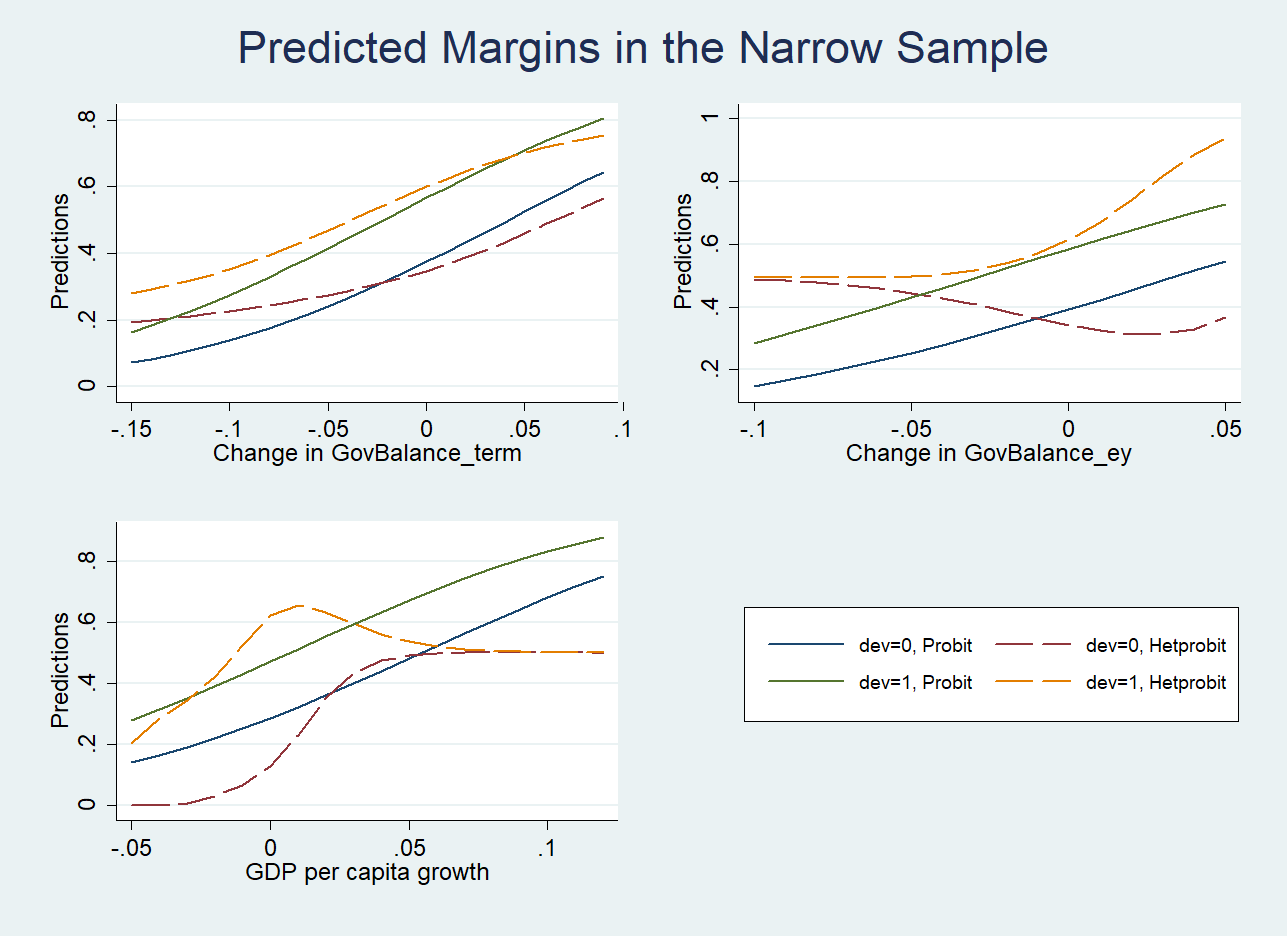
\includegraphics[width=1\textwidth]{Predicted_Narrow.png}

\end{figure}

\end{frame}
%--------------------------------------------------------------
\begin{frame}
 \begin{figure}
    \centering
    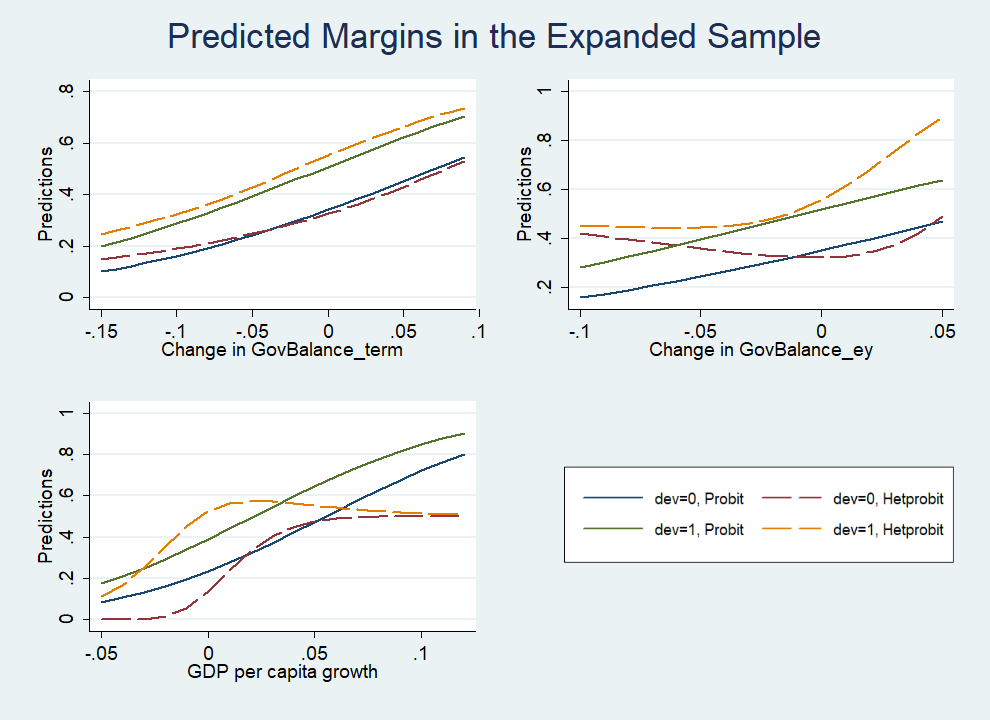
\includegraphics[width=1\textwidth]{Predicted_Expanded.png}

\end{figure}   
\end{frame}
%--------------------------------------------------------------
\begin{frame}
    \begin{figure}
        \centering
        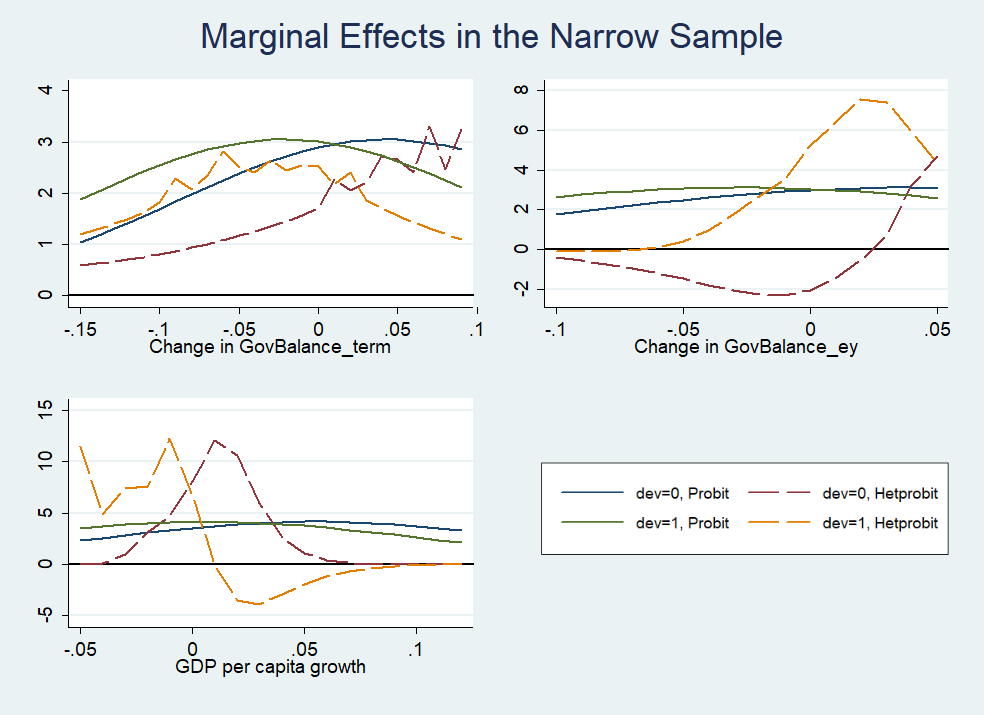
\includegraphics[width=1\textwidth]{AME_Narrow.png}
        \caption{Caption}
        \label{fig:my_label}
    \end{figure}
\end{frame}
%--------------------------------------------------------------
\begin{frame}
    \begin{figure}
        \centering
        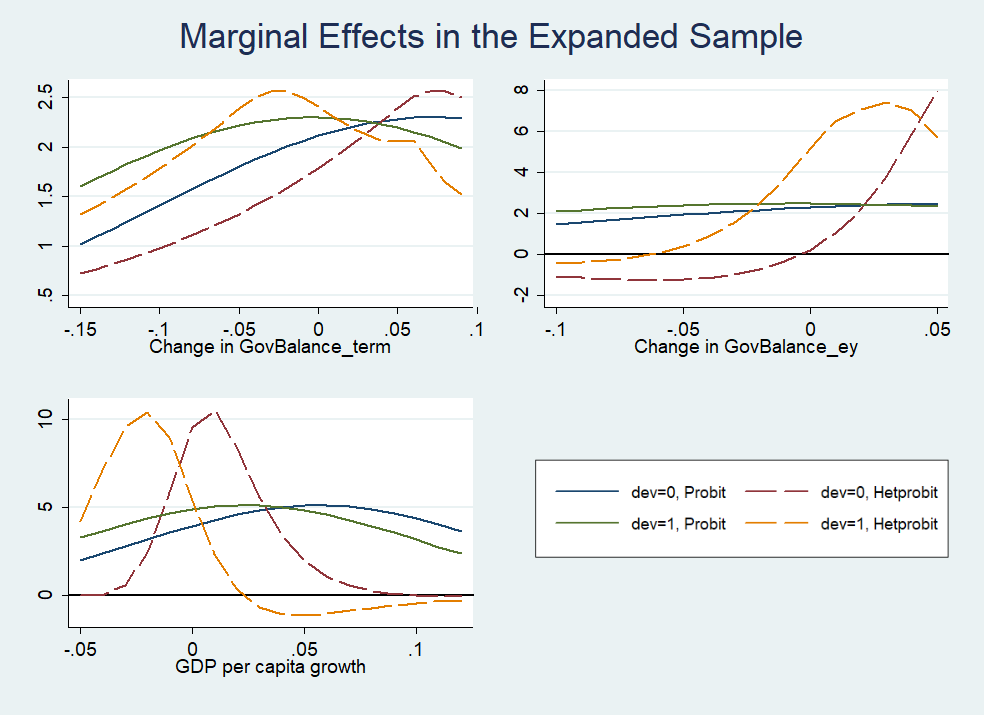
\includegraphics[width=1\textwidth]{AME_expanded.png}
        \caption{Caption}
        \label{fig:my_label}
    \end{figure}
\end{frame}
%--------------------------------------------------------------
\begin{frame}{Conclusion}
\setlength\itemsep{2em}
\begin{enumerate}
\setlength\itemsep{2em}
    \item \textit{Does more growth lead to a higher reelection chance?} 
    \item \textit{Does improvement in the government balance lead to a higher chance in reelection?}\pause
\end{enumerate}
\item\underline{Answer:} \textbf{Generally yes, but not always...}
\end{frame}
\end{document}
\end{document}